

% Este é um documento de amostra simples. Para documentos mais complicados, dê uma olhada na aba de exercícios. Note que tudo que vem depois de um símbolo % é tratado como comentário e ignorado quando o código é compilado.

\documentclass[ 12pt,a4paper ]{article} % \documentclass{} é o primeiro comando em qualquer código LaTeX. Ele é usado para definir que tipo de documento você está criando, como um artigo ou um livro, e inicia o preâmbulo do documento

% --- PACOTES DE LÍNGUA E CODIFICAÇÃO ---
\usepackage[portuguese]{babel}  % Configurar idioma para português
\usepackage[utf8]{inputenc}
\usepackage[T1]{fontenc}

% --- PACOTES DE MATEMÁTICA E COMANDOS ---
\usepackage{amsmath, amssymb, amsthm}
\usepackage{bm} 
\usepackage{mathtools} % Extensão do amsmath para dcases (opcional)
\usepackage{bigints} % Adicione este pacote
\newcommand{\N}{\mathbb{N}}
\newcommand{\R}{\mathbb{R}}
\newcommand{\E}{\mathbb{E}}
\newcommand{\Prob}{\mathbb{P}}
\newcommand{\Var}{\mathrm{Var}}
\newcommand{\Cov}{\mathrm{Cov}}

% --- AMBIENTES DE TEOREMA ---
\newtheorem{theorem}{Teorema}
\newtheorem{lemma}{Lema}
\newtheorem{corollary}{Corolário}
\newtheorem{proposition}{Proposição}
%\theoremstyle{definition}
\newtheorem{definition}{Definição}
\newtheorem{example}{Exemplo}
\newtheorem{remark}{Observação}


% --- PACOTES DE FORMATAÇÃO E LAYOUT ---
\usepackage[left=3cm,right=2cm,top=3cm,bottom=2cm]{geometry}
% Pacote para personalizar cabeçalhos e rodapés
\usepackage{fancyhdr}
\usepackage{graphicx}
\usepackage{booktabs} % Para melhorar a aparência das tabelas
\usepackage{caption}  % Para customizar legendas
\usepackage{longtable}
\usepackage{setspace}

% --- BIBLIOGRAFIA (usando Biblatex) ---alphabetic
\usepackage[backend=biber, style=numeric, natbib=true, backref=true, sorting=nty]{biblatex}
\addbibresource{referencias.bib} % Declare seu arquivo .bib aqui (com a extensão!)

% --- HYPERREF (deve ser um dos últimos pacotes a ser carregado) ---
\usepackage{hyperref}
\hypersetup{
	colorlinks=true,
	citecolor=red,
	linkcolor=blue,
	filecolor=magenta,
	urlcolor=cyan,
}

% --- CONFIGURAÇÕES DE ESPAÇAMENTO E CABEÇALHO ---
\onehalfspacing %Para um espaçamento de 1,5
%\doublespacing % Para um espaçamento duplo
\pagestyle{fancy}
%\bibliographystyle{apalike}
%\bibliographystyle{abbrv}
\fancyhf{} % Limpa cabeçalhos e rodapés padrão
%\fancyhead[L]{Texto à esquerda do cabeçalho} % Cabeçalho à esquerda
\fancyhead[C]{Programa Interinstitucional de Pós-Graduação em Estatística UFSCar-USP (PIPGEs)\\
	Doutorado em Estatística} % Cabeçalho centralizado
%\fancyhead[R]{Texto à direita do cabeçalho} % Cabeçalho à direita
\title{\textbf{Modelagem Preditiva de Níveis de Rio Utilizando um Modelo SARIMAX em forma de Espaço de Estado}} % Define o título do artigo
\author{Professor: Vicente Garibay Cancho\\
Discente: Edfram Rodrigues Pereira} 
%\author{Discente: Edfram Rodrigues Pereira} % Define o nome do autor
\date{\today} % Define a data para a data compilada

% O preâmbulo termina com o comando \begin{document}
	\begin{document} % Todos os comandos begin devem ser pareados com um comando end em algum lugar
		\maketitle % cria um título usando informações no preâmbulo (título, autor, data)
		% Aplica o cabeçalho na primeira página
		\thispagestyle{fancy}
		
		\begin{abstract}
		
		A acentuada sazonalidade hidrológica do Rio Solimões impõe severos desafios socioeconômicos à Bacia Amazônica, tornando a previsão de seus níveis uma ferramenta essencial para a gestão de riscos. Este estudo propõe o desenvolvimento e a avaliação de um modelo Sazonal Autorregressivo Integrado de Médias Móveis com Variáveis Exógenas (SARIMAX) para a previsão de médio prazo (1 a 4 meses) dos níveis do rio em Tabatinga-AM. Utilizando dados mensais de nível (variável endógena) e vazão (variável exógena) de 1995 a 2024, a metodologia abrange uma rigorosa análise exploratória, incluindo testes formais para verificação de sazonalidade (Kruskal-Wallis) e estacionariedade (Dickey-Fuller Aumentado). O modelo é implementado em um framework de espaço de estados, com um tratamento específico para outliers a fim de aumentar sua robustez. O objetivo é fornecer um modelo estatístico acurado e confiável que possa subsidiar a tomada de decisão estratégica por órgãos de defesa civil e outros agentes envolvidos na gestão de recursos hídricos na região.
		
	\end{abstract}
	
	% Adicionando Palavras-chave (opcional, mas comum)
	\noindent % Impede a indentação da primeira linha
	\textbf{Palavras-chave:} Séries Temporais, Modelo SARIMAX, Previsão, Hidrologia, Espaço de Estado.
	
	\vspace{1cm} % Adiciona um espaço vertical antes do início do conteúdo
		
		\section{Introdução}%
		\label{sect:intro}
		
		Os rios da Bacia Amazônica, com destaque para o Rio Solimões, um dos principais formadores do Rio Amazonas, são sistemas hidrológicos complexos e dinâmicos que sustentam uma biodiversidade ímpar e são cruciais para o modo de vida e a economia de milhões de pessoas. A marcante sazonalidade hidrológica, caracterizada por amplos e recorrentes pulsos de inundação ~\cite{SCHONGART2007} e, cada vez mais, por eventos de seca severa, impõe desafios socioeconômicos significativos. Nesse contexto, a capacidade de realizar previsões acuradas das séries temporais de níveis d'água no Rio Solimões assume um papel de vital importância para a mitigação de desastres naturais, o planejamento de atividades econômicas e a gestão sustentável dos vastos recursos hídricos da região.
		
		O fenômeno da cheia nos rios amazônicos é um evento natural que molda a paisagem e os ecossistemas de várzea. No entanto, quando as inundações atingem magnitudes extremas, transformam-se em desastres socioambientais. As cheias podem resultar no desalojamento de comunidades ribeirinhas, perdas na agricultura de subsistência e comercial, danos a infraestruturas urbanas e rurais, interrupção de vias de transporte fluvial – essenciais na Amazônia – e aumento da incidência de doenças de veiculação hídrica ~\cite{alves2022}, ~\cite{LIU2023}. A implementação e o aprimoramento de sistemas de alerta, como analisado por ~\cite{Maciel2022} para o Rio Negro, e a capacidade de prever a magnitude e o timing das cheias com dias ou semanas de antecedência ~\cite{SIQUEIRA2020} são, portanto, cruciais para permitir a adoção de medidas preventivas, como a remoção de populações de áreas de risco e a proteção de bens, minimizando perdas humanas e materiais.
		
		Em contrapartida, os eventos de seca no Rio Solimões e em outros grandes rios amazônicos têm se tornado mais frequentes e intensos, exacerbados por variabilidades climáticas e possíveis mudanças ambientais. Níveis d'água excessivamente baixos comprometem severamente a navegação, que representa a principal via de transporte de pessoas e mercadorias para inúmeras localidades, isolando comunidades e encarecendo produtos essenciais. Além disso, as secas afetam o abastecimento de água para consumo humano, a atividade pesqueira – fundamental para a segurança alimentar e renda local –, a agricultura nas áreas de terra firme e várzea, e podem impactar a geração de energia em sistemas isolados ou interligados que dependem de fontes hídricas. A previsão de níveis mínimos com meses de antecedência, utilizando indicadores climáticos como os índices ENSO ~\cite{SCHONGART2007}, ~\cite{Chevuturi2021} ou previsões sazonais de modelos climáticos ~\cite{Gubler2020}, é vital para o planejamento estratégico do uso da água, a gestão de hidrovias e a preparação para contingências.
		
		Diante da relevância socioeconômica dos ciclos de cheia e seca, a previsão de séries temporais de níveis d'água para o Rio Solimões é uma ferramenta indispensável. Previsões confiáveis, abrangendo diferentes horizontes temporais – desde curto prazo, em horas ~\cite{LIU2023}, médio prazo, em dias ~\cite{Nguyen2015}, ~\cite{Duque2022}, até longo prazo, em meses ~\cite{SCHONGART2007}, ~\cite{Gubler2020} – subsidiam a tomada de decisão em múltiplos setores. Defesas civis, órgãos gestores de recursos hídricos, operadores de portos, empresas de navegação, agricultores e a população em geral podem se beneficiar diretamente dessas informações para otimizar suas atividades e reduzir sua vulnerabilidade.
		
		A complexidade da bacia amazônica e a interação de diversos fatores climáticos e hidrológicos tornam a previsão uma tarefa desafiadora. Por isso, uma diversidade de abordagens metodológicas tem sido investigada, desde modelos hidrológicos e hidrodinâmicos que buscam representar os processos físicos ~\cite{fan2021}, ~\cite{SIQUEIRA2020}, passando por modelos estatísticos que exploram relações com preditores climáticos ~\cite{Chevuturi2021}, ~\cite{Gubler2020}, até o uso crescente de técnicas de aprendizado de máquina ~\cite{Nguyen2015}, ~\cite{Duque2022}, ~\cite{LIU2023} que demonstram grande potencial para capturar relações não-lineares complexas.
		
		Este trabalho se propõe a desenvolver e avaliar o modelo SARIMAX via modelo de espaço de estado para previsão de nível d'água do Rio Solimões em Tabatinga, com foco em horizontes de previsão de 1 a 4 meses. Ao buscar aprimorar a capacidade de antecipação das variações dos níveis do Rio Solimões, espera-se contribuir para a redução dos impactos socioeconômicos adversos associados aos eventos hidrológicos extremos na Amazônia e fomentar uma gestão mais resiliente e adaptativa dos recursos hídricos.
		
		%Este trabalho se propõe a desenvolver e avaliar modelos estatísticos de previsão de nível máximo e mínimo anual de água do Rio Solimões em Tabatinga, avaliar e comparar diferentes modelos de aprendizado de máquina para a previsão de níveis diários do Rio Solimões em Tabatinga-AM, com foco em horizontes de previsão de 1 a 3 meses. Ao buscar aprimorar a capacidade de antecipação das variações dos níveis do Rio Solimões, espera-se contribuir para a redução dos impactos socioeconômicos adversos associados aos eventos hidrológicos extremos na Amazônia e fomentar uma gestão mais resiliente e adaptativa dos recursos hídricos.
		
		%" OU "desenvolver um sistema híbrido de previsão de cheias para o Rio Solimões, combinando modelos hidrológicos com dados de sensoriamento remoto."].
		
		\subsection{Trabalhos Relacionados}%
		\label{ssect:cit-ref}%
		\index{citação}
		%Uma análise comparativa de dez estudos recentes na área de previsão hidrológica e hidrometeorológica revela uma diversidade significativa de abordagens metodológicas, métricas de avaliação, horizontes de previsão e contribuições para o avanço do conhecimento. Os trabalhos de ~\cite{Maciel2022}, ~\cite{alves2022}, ~\cite{Gubler2020}, ~\cite{Chevuturi2021}, ~\cite{SCHONGART2007}, ~\cite{Nguyen2015}, ~\cite{Duque2022}, ~\cite{LIU2023}, ~\cite{fan2021} e ~\cite{SIQUEIRA2020} foram considerados nesta síntese.
		
		No que tange às metodologias utilizadas, observa-se %um espectro amplo. Modelos com base física ou hidrodinâmica são empregados por ~\cite{fan2021} e ~\cite{alves2022} e ~\cite{SIQUEIRA2020}. Os primeiros utilizam o modelo MGB, focando no mapeamento de áreas de perigo e no impacto da discretização da rede de drenagem, enquanto o último combina saídas de modelos de previsão de tempo por ensemble com o modelo hidrodinâmico CaMa-Flood para previsões em escala continental. Em contraste, 
		abordagens puramente estatísticas ou baseadas em indicadores climáticos como em ~\cite{Gubler2020}, que avaliam o desempenho do sistema de previsão sazonal SEAS5; ~\cite{Chevuturi2021}, que utilizam regressão múltipla para prever cotas máximas anuais; e ~\cite{SCHONGART2007}, que aplicam regressão linear com índices ENSO para prever o pulso de cheia. Uma outra vertente metodológica proeminente é a de \textit{machine learning}, explorada por ~\cite{Nguyen2015} que comparam LASSO, Random Forests e Support Vector Regression (SVR); ~\cite{Duque2022} que implementam uma rede Perceptron Multicamadas (MLP) com dados de múltiplas estações; e ~\cite{LIU2023} que contrastam Redes Neurais Recorrentes (RNN) clássicas, Gated Recurrent Units (GRU) e Long Short-Term Memory (LSTM), demonstrando a superioridade desta última para previsões em resolução horária. Finalmente, ~\cite{Maciel2022} focam na análise de um sistema de alerta operacional, investigando tempos de viagem da onda de cheia e propondo melhorias.
		
		%As medidas de performance adotadas para análise de resultados também variam consideravelmente. Métricas hidrológicas clássicas como o Coeficiente de Eficiência de Nash-Sutcliffe (NSE), o Kling-Gupta Efficiency (KGE) e a Raiz do Erro Quadrático Médio (RMSE) são comuns em estudos como os de ~\cite{alves2022}, ~\cite{Duque2022}, ~\cite{LIU2023} e ~\cite{fan2021}. O Erro Absoluto Médio (MAE) foi utilizado por ~\cite{Nguyen2015}. Para avaliações de previsões por ensemble ou probabilísticas, métricas como o Continuous Ranked Probability Skill Score (CRPSS), Brier Skill Score (BSS) e a Receiver Operating Characteristic (ROC) são empregadas por ~\cite{Gubler2020}, ~\cite{Chevuturi2021} e ~\cite{SIQUEIRA2020}. Indicadores específicos para mapas de inundação, como o False Alarm Ratio (FAR) e o Critical Success Index (CSI), aparecem no trabalho de ~\cite{alves2022}, enquanto a avaliação do erro no pico da cheia (seja em magnitude, \(\Delta H\), ou no tempo de ocorrência) é crucial para ~\cite{Maciel2022} e ~\cite{LIU2023}.
		
		O horizonte de previsão e a seleção de preditores são intrinsecamente ligados à metodologia e aos objetivos de cada estudo. Para previsões de curtíssimo prazo (1 a 12 horas), ~\cite{LIU2023} utilizam dados de vazão e nível da própria bacia. Em horizontes de alguns dias (1 a 15 dias), ~\cite{Maciel2022}, ~\cite{alves2022}, ~\cite{Nguyen2015}, ~\cite{Duque2022} e ~\cite{SIQUEIRA2020} empregam combinações de dados de chuva, níveis observados, saídas de modelos atmosféricos por ensemble e lags temporais das variáveis hidrológicas. Para previsões com antecedência de meses (4 a 8 meses), ~\cite{SCHONGART2007} baseiam-se em índices ENSO como o SOI e Niño3.4. Previsões sazonais (1 a 6 meses) são o foco de ~\cite{Gubler2020}, que utilizam diretamente as saídas do modelo SEAS5. A previsão da cota máxima anual, investigada por ~\cite{Chevuturi2021}, recorre a índices climáticos globais (ENSO, PDO) e projeções de precipitação. Por fim, o estudo de ~\cite{fan2021} sobre a discretização da rede fluvial analisa simulações contínuas para um período climatológico base, focando no impacto de parâmetros como \(\Delta x\) e o número de Courant-Friedrichs-Lewy (CFL).
		
		%Os principais resultados demonstram avanços significativos em diversas frentes. Em previsões de curta escala, ~\cite{LIU2023} alcançaram NSE superior a 0,98 e RMSE inferior a 0,2 m com LSTM, enquanto ~\cite{Nguyen2015} mostraram que o SVR pode atender aos requisitos da Comissão do Rio Mekong com MAE de 0,486 m. ~\cite{Duque2022} observaram um decaimento do NSE de 0,93 para 0,54 ao aumentar o horizonte de previsão de 1 para 7 dias. No mapeamento de inundações, ~\cite{alves2022} reproduziram aproximadamente 70\% das áreas com profundidade superior a 1 m, embora com limitações em terrenos planos. ~\cite{SIQUEIRA2020} mostraram que previsões hidrológicas por ensemble em escala continental podem agregar valor (CRPSS > 0) em cerca de 60\% das seções analisadas. ~\cite{Gubler2020} identificaram habilidade preditiva do SEAS5 (ACC > 0,3) para precipitação no noroeste da Amazônia. ~\cite{SCHONGART2007} obtiveram R² de aproximadamente 0,6 na previsão da cota de pico na Amazônia Central utilizando índices ENSO. ~\cite{Chevuturi2021} conseguiram uma redução de 25\% no erro da previsão da cota máxima anual. ~\cite{fan2021} concluíram que uma discretização espacial (\(\Delta x\)) inferior ou igual a 15 km, combinada com um limitador de Froude, equilibra custo computacional e estabilidade numérica. ~\cite{Maciel2022} demonstraram um ganho operacional de 20-30\% na antecedência do aviso de cheia com ajustes no sistema existente.
		
		As contribuições desses estudos são variadas e impactantes. Trabalhos como os de ~\cite{LIU2023} e ~\cite{Nguyen2015} avançam na aplicação de técnicas de \textit{Deep Learning} e \textit{Machine Learning} para previsão hidrológica. ~\cite{alves2022} e ~\cite{fan2021} e ~\cite{SIQUEIRA2020} trazem progressos na modelagem hidrológica e hidrodinâmica em larga escala com foco na consistência física e aplicabilidade. ~\cite{Gubler2020}, ~\cite{Chevuturi2021} e ~\cite{SCHONGART2007} fortalecem a ponte entre climatologia e hidrologia, explorando a previsibilidade em escalas sazonais a anuais. Por fim, o estudo de ~\cite{Maciel2022} ressalta a importância da calibração e otimização de sistemas de alerta operacionais, mostrando que ganhos significativos podem ser obtidos através de análises focadas e ajustes metodológicos.
		
		Em síntese, a literatura recente sobre previsão de cheias e níveis d'água exibe métodos e escalas de aplicação, refletindo os desafios e as oportunidades para melhorar a capacidade de antecipação e mitigação de eventos hidrológicos extremos. A combinação de modelos baseados em processos físicos, abordagens estatísticas avançadas e o crescente poder do aprendizado de máquina oferece um panorama promissor para o futuro da previsão hidrológica.
		
%		\begin{table}[htbp]
%			\centering
%			
%			\caption{Tabela-resumo comparativa de estudos em previsão hidrológica.}
%			\label{tab:comparativa_sem_id}
%			\begin{tabular}{|p{2.5cm}|p{2.5cm}|p{2.0cm}|p{1.5cm}|p{2.5cm}|p{3.0cm}|}
%				\hline
%				\textbf{Artigo (1ª autora, ano)} & \textbf{Metodologia principal} & \textbf{Métricas usadas} & \textbf{Horizonte} & \textbf{Preditores chave} & \textbf{Principais achados} \\
%				\hline
%				Maciel 2022 – “Analysing the flood warning of Negro river in Manaus” & Sistema de alerta; checagem do tempo-de-viagem da onda; análises estatísticas clássicas & NSE, RMSE, Erro pico & 1–10 d & Chuva, nível e tempo de viagem & Ganho de 20–30\% na antecedência do aviso em relação ao sistema operacional \\
%				\hline
%				Alves 2022 – “Assessing the capacity of large-scale hydrologic-hydrodynamic models for mapping flood hazard in southern Brazil” & MGB+inércia local (1D); calibração multi-bacia & NSE, KGE, RMSE, FAR/CSI para mapas de inundação & Eventos anuais (1997–2020) & Chuva satélite, rede de calha vetorial & Reprod. de 70\% das áreas inundadas $>$ 1 m de profundidade \\
%				\hline
%				Gubler 2022 – “Assessment of ECMWF SEAS5 Seasonal Forecast Performance over South America” & Avaliação estatística de previsões sazonais (SEAS5) & ACC, CRPSS, BSS, ROC & 1–6 meses (DJF, MAM, etc.) & Campos do modelo SEAS5 & Habilidade $>$ 0,3 (ACC) no NW da Amazônia para precipitação \\
%				\hline
%				Chevuturi 2021 – “Forecasting annual maximum water level for the Negro River at Manaus” & Regressão múltipla + preditores climáticos + hindcasts & $\rho$ de Pearson, CRPSS & 1 ano & ENSO, PDO, precipitação projetada & Redução de 25\% no erro da cota máxima anual \\
%				\hline
%				Schöngart 2004 – “Forecasting the flood-pulse in Central Amazonia by ENSO-indices” & Regressão linear simples/múltipla entre SOI e água ref. Manaus & R$^2$, RMSE & 4–8 meses & SOI, Niño3.4, ONI & R$^2 \approx$ 0,6 na previsão da cota de pico \\
%				\hline
%				Nguyen 2019 – "Forecasting Time Series Water Levels on Mekong River Using Machine Learning Models" & LASSO, RF, SVR & MAE, RMSE, CE & 5 d & Lags de nível (2 estações) & SVR: MAE = 0,486 m ($<$ limite MRC) \\
%				\hline
%				Duque 2022 – "Level river forecasting using empirical hydrological modeling for Rio Negro basin Uruguay" & Perceptron 38-18-1 & NSE, RMSE & 1–7 d & Nível + chuva (19 est.) & NSE: 0,93 (1 d) $\rightarrow$ 0,54 (7 d) \\
%				\hline
%				Liu 2023 – "Long Short-Term Memory (LSTM) Based Model for Flood Forecasting in Xiangjiang River" & RNN $\times$ GRU $\times$ LSTM & NSE, RMSE, $\Delta$H pico & 1 h, 6 h, 12 h & Vazão(a)/nível(u) & LSTM: NSE $>$ 0,98; RMSE $<$ 0,2 m \\
%				\hline
%				Fan 2021 – “On the discretization of river networks for large scale hydrologic-hydrodynamic models” & Experimentos $\Delta$x fixo (5–50 km) no MGB & NSE, KGE, erro balanço & Simulação contínua 1998-2010 & $\Delta$x, CFL, Froude-limiter & $\Delta$x $\leq$ 15 km equilibra custo e estabilidade \\
%				\hline
%				Siqueira 2020 – “Potential skill of continental-scale, medium-range ensemble streamflow forecasts for flood prediction in South America” & ECMWF-ENS + CaMa-Flood & CRPS, BSS, hit/falsos & 1–15 d & Saídas do ENS + peaking rule & CRPSS $>$ 0 em 60\% das seções ($>$ 30\% área) \\
%				\hline
%			\end{tabular}
%		\end{table}
		
		%\section*{Exemplo de Tabela Longa}
		%\normalsize
		%\footnotesize
%		{
%		\fontsize{6pt}{8pt}
%		\begin{longtable}{|p{2.5cm}|p{2.5cm}|p{1.8cm}|p{2cm}|p{2.2cm}|p{3.0cm}|}%{llllll}
%			%\footnotesize % Adjust font size to make the table fit
%			\caption{Tabela-resumo comparativa de estudos em previsão hidrológica.} \label{tab:minha_longa_tabela} \\
%			\toprule % Linha superior do booktabs
%			Artigo (1ª autora, ano) & Metodologia principal & Métricas usadas & Horizonte & Preditores chave & Principais achados \\
%			\midrule % Linha abaixo do cabeçalho do booktabs
%			\endfirsthead % Fim do cabeçalho da primeira página
%			
%			\multicolumn{6}{c}%
%			{{\bfseries }} \\ % Título de continuação
%			\toprule
%			Artigo (1ª autora, ano) & Metodologia principal & Métricas usadas & Horizonte & Preditores chave & Principais achados \\
%			\midrule
%			\endhead % Fim do cabeçalho das páginas seguintes
%			
%			\midrule
%			\multicolumn{6}{r}{{Continua na próxima página}} \\
%			\bottomrule
%			\endfoot % Fim do rodapé das páginas intermediárias
%			
%			\bottomrule
%			\endlastfoot % Fim do rodapé da última página
%			
%			% Dados da tabela (adicione muitas linhas para testar)
%			Maciel 2022-“Analysing the flood warning of Negro river in Manaus” & Sistema de alerta; checagem do tempo-de-viagem da onda; análises estatísticas clássicas & NSE, RMSE, Erro pico & 1–10 d & Chuva, nível e tempo de viagem & Ganho de 20–30\% na antecedência do aviso em relação ao sistema operacional \\
%			\hline
%			Alves 2022-“Assessing the capacity of large-scale hydrologic-hydrodynamic models for mapping flood hazard in southern Brazil” & MGB+inércia local (1D); calibração multi-bacia & NSE, KGE, RMSE, FAR/CSI para mapas de inundação & Eventos anuais (1997–2020) & Chuva satélite, rede de calha vetorial & Reprod. de 70\% das áreas inundadas $>$ 1 m de profundidade \\
%			\hline
%			Gubler 2022-“Assessment of ECMWF SEAS5 Seasonal Forecast Performance over South America” & Avaliação estatística de previsões sazonais (SEAS5) & ACC, CRPSS, BSS, ROC & 1–6 meses (DJF, MAM, etc.) & Campos do modelo SEAS5 & Habilidade $>$ 0,3 (ACC) no NW da Amazônia para precipitação \\
%			\hline
%			Chevuturi 2021-“Forecasting annual maximum water level for the Negro River at Manaus” & Regressão múltipla + preditores climáticos + hindcasts & $\rho$ de Pearson, CRPSS & 1 ano & ENSO, PDO, precipitação projetada & Redução de 25\% no erro da cota máxima anual \\
%			\hline
%			Schöngart 2004-“Forecasting the flood-pulse in Central Amazonia by ENSO-indices” & Regressão linear simples/múltipla entre SOI e água ref. Manaus & R$^2$, RMSE & 4–8 meses & SOI, Niño3.4, ONI & R$^2 \approx$ 0,6 na previsão da cota de pico \\
%			\hline
%			Nguyen 2019-"Forecasting Time Series Water Levels on Mekong River Using Machine Learning Models" & LASSO, RF, SVR & MAE, RMSE, CE & 5 d & Lags de nível (2 estações) & SVR: MAE = 0,486 m ($<$ limite MRC) \\
%			\hline
%			Duque 2022-"Level river forecasting using empirical hydrological modeling for Rio Negro basin Uruguay" & Perceptron 38-18-1 & NSE, RMSE & 1–7 d & Nível + chuva (19 est.) & NSE: 0,93 (1 d) $\rightarrow$ 0,54 (7 d) \\
%			\hline
%			Liu 2023-"Long Short-Term Memory (LSTM) Based Model for Flood Forecasting in Xiangjiang River" & RNN $\times$ GRU $\times$ LSTM & NSE, RMSE, $\Delta$H pico & 1 h, 6 h, 12 h & Vazão(a)/nível(u) & LSTM: NSE $>$ 0,98; RMSE $<$ 0,2 m \\
%			\hline
%			Fan 2021-“On the discretization of river networks for large scale hydrologic-hydrodynamic models” & Experimentos $\Delta$x fixo (5–50 km) no MGB & NSE, KGE, erro balanço & Simulação contínua 1998-2010 & $\Delta$x, CFL, Froude-limiter & $\Delta$x $\leq$ 15 km equilibra custo e estabilidade \\
%			\hline
%			Siqueira 2020-“Potential skill of continental-scale, medium-range ensemble streamflow forecasts for flood prediction in South America” & ECMWF-ENS + CaMa-Flood & CRPS, BSS, hit/falsos & 1–15 d & Saídas do ENS + peaking rule & CRPSS $>$ 0 em 60\% das seções ($>$ 30\% área) \\
%			\hline
%		\end{longtable}
%	}
	
	\section{Metodologia e Modelagem}
	
	Nosso objetivo é fazer previsão de nível d'água do rio Solimões (variável endógena), na região da cidade de Tabatinga-AM com lag de 4 meses, considerando como variável exógena a vazão do rio. A base de dados consistiu em uma série temporal de nível d'água do rio Solimões (\textit{nivel}), medida em $cm$, e outra de vazão afluente (\textit{vazao}), medida em $m^3/s$. As séries são constituídas de dados mensais do período de $01/01/1995$ a $01/03/2024$, ou seja, 350 linhas de dados. Os dados foram obtidos da estação portuária de Tabatinga-AM (ID: 10100000) sob a responsabilidade da Agência Nacional de Águas-ANA e disponibilizados no site Sistema Nacional de Informações sobre Recursos Hídricos (SNIRH)\footnote{ https://www.snirh.gov.br/hidroweb/serieshistoricas}.
	 
	%Com o intuito de aplicar o modelo $SARIMAX$ foi realizado o teste Breusch-Pagan com o intuito de verificar se a série apresenta homoscedasticidade, requisito fundamental para que tenhamos resultados confiáveis.  
	
	\subsection{Análise Exploratória de Dados (AED)}
	
	Realizamos uma verificação das principais estatísticas descritiva dos dados com intuito de ter a primeira impressão do mesmo. Plotamos a série temporal e sua decomposição sazonal para verificar de forma visual se há tendência e/ou sazonalidade. Criamos boxplots por mês para verificar  outilier e a sazonalidade anual, que também foi verificada através do teste de Kruskal. Testamos a estacionariedade da série com o teste de Dickey-Fuller Aumentado.
	
	
	\subsubsection{Teste de Kruskal-Wallis para Sazonalidade}
	
	O Teste de Kruskal-Wallis (1952)~\cite{Kruskal} é um teste estatístico não paramétrico, ou seja, não assume que os dados seguem uma distribuição específica. Seu objetivo é determinar se as amostras de dois ou mais grupos independentes se originam da mesma distribuição. Em vez de ver a série temporal como uma sequência contínua, agrupamos de acordo com o período sazonal que queremos testar.
	O teste, então, não analisa o "tempo", mas sim se a distribuição dos valores é a mesma em todos esses grupos (meses).
	
	\begin{itemize}
		
	
	\item  \textbf{Hipóteses do Teste no Contexto de Sazonalidade}
	
	\begin{itemize}
		
	
	\item \textit{Hipótese Nula ($H_0$)}: Não há sazonalidade.
	
	A distribuição dos valores é a mesma para todos os períodos (meses). Qualquer diferença observada entre as medianas dos grupos é devida ao acaso.
	
	\item \textit{Hipótese Alternativa ($H_1$)}: Há sazonalidade.
	
	Pelo menos um período tem uma distribuição de valores diferente dos outros. Isso implica que o período do ano tem um efeito sistemático sobre o valor da variável.
\end{itemize}
	\item Os Passos Matemáticos 
	
	\begin{enumerate}
		\item Agrupar e Rankear os Dados
		
		Separe as observações em $k$ grupos (sazonalidade mensal, $k=12$).
		Junte todas as observações de todos os grupos em uma única lista e atribua ranks a elas, do menor valor para o maior. A menor observação recebe rank 1, a segunda menor recebe rank 2, e assim por diante.
		
		\item Calcular a Estatística de Teste (H)
		
		A estatística $H$ mede a soma das diferenças entre os ranks médios de cada grupo e o rank médio geral. Se os grupos vierem da mesma população, seus ranks médios devem ser muito parecidos.
		
		A fórmula é: $$H = \left[\dfrac{12}{N(N+1)} \sum_{1}^{k}\dfrac{R_i^2}{n_i}\right] - 3 (N+1)$$
		
		Onde:
		\begin{itemize}
			
		
		\item $N$: O número total de observações (em todos os grupos).
		
		\item $k$: O número de grupos (ex: 12 para meses).
		
		\item $n_i$: O número de observações no grupo i.
		\item $R_i$: A soma dos ranks no grupo i.
		
		\end{itemize}
		
		\item Tomar a Decisão Estatística
		
		Sob a hipótese nula ($H_0$), a estatística $H$ segue aproximadamente uma distribuição Qui-quadrado ($\chi^2$) com $k-1$ graus de liberdade (onde $k$ é o número de grupos).
		O p-valor é a probabilidade de obter um valor de $H$ tão extremo ou maior do que o que foi calculado, assumindo que não há sazonalidade.
		Usando um nível de significância $\alpha$ (geralmente 0.05):
		
		Se p-valor  $ <\alpha$: Rejeitamos a hipótese nula ($H_0$). Há evidência estatística de sazonalidade.
		
		Se p-valor $\geq \alpha$: Não rejeitamos a hipótese nula ($H_0$). Não há evidência estatística de sazonalidade.
		
	\end{enumerate}
\end{itemize}
	
	\subsubsection{Teste de Dickey-Fuller Aumentado (DFA) para Estacionariedade}
	
	O teste DFA (Dickey \& Fuller, 1979, 1981)~\cite{Dickey1},~\cite{Dickey2} verifica se uma série temporal precisa ser diferenciada para se tornar estacionária. Ele testa a presença de uma 'raiz unitária'.
	
	Consideremos uma série temporal como um passeio aleatório:
	$$y_t=y_{t-1} + \epsilon_t$$
	Onde $\epsilon_t$ é um ruído branco (um choque aleatório). Nesta equação, o valor de hoje ($y_t$) é simplesmente o valor de ontem ($y_{t-1}$) mais um passo aleatório. Um choque ($\epsilon_t$) nesta série é permanente. Ele é incorporado para sempre e a série nunca retorna a uma média. Isso é uma raiz unitária.
	
	Agora, considere uma série estacionária (um processo AR(1)):
		$$y_t= \rho y_{t-1} + \epsilon_t$$

	onde $|\rho |<1$
	
	Aqui, o valor de ontem é descontado por um fator $\rho$. Um choque nesta série é temporário e seu efeito decai com o tempo. A série sempre tende a retornar à sua média.
	
	O teste DFA tenta descobrir em qual desses dois cenários a série temporal vive.
	
	\begin{itemize}
		\item \textbf{Hipóteses do Teste}
		
			\begin{itemize}
		\item \textit{Hipótese Nula ($H_0$)}: A série possui uma raiz unitária ($\delta=0$).
		
		Isso significa que a série é não estacionária.
		
		\item \textit{Hipótese Alternativa ($H_1$)}: A série não possui uma raiz unitária ($\delta<0$).
		
		Isso significa que a série é estacionária (ou estacionária em torno de uma tendência).
			\end{itemize}
			
		\item Os Passos Matemáticos
		
		\begin{enumerate}
			\item Construir a Equação de Regressão do Teste
			
			O teste executa uma regressão de Mínimos Quadrados Ordinários (OLS) na seguinte forma:
			
			$$\Delta y_t= \alpha + \beta_t + \delta y_{t-1} + \sum_{i=1}^{p} \gamma_i \Delta y_{t-1} +\epsilon_t $$
			
			Onde:
			\begin{itemize}
				
				\item $\Delta y_t$: a série diferenciada ($y_t- y_{t-1}$). É a variável dependente.
				
				\item $y_{t-1}$: a série original defasada em um período. É a variável chave do teste.
				
				\item $\delta$: o coeficiente de $y_{t-1}$.  É neste coeficiente que o teste se concentra. Se  $\delta=0$, a equação original tinha uma raiz unitária.
				
				\item $\alpha$: uma constante.
				
				\item $\beta_t$: um termo de tendência temporal.
				
				\item $\sum_{i=1}^{p} \gamma_i \Delta y_{t-1}$: Os termos 'aumentados'. São as diferenças defasadas que capturam qualquer correlação serial (autocorrelação) nos resíduos, garantindo que 	$\epsilon_t $ seja ruído branco. O número de defasagens $p$ é escolhido usando critérios de informação como AIC ou BIC.
			\end{itemize}
			
			\item Calcular a Estatística de Teste
			
			Após rodar a regressão, obtemos o valor do coeficiente $\delta$ e seu erro padrão. A estatística de teste (chamada de estatística DFA) é calculada como:
			
			$$DFA_{stat}	= \dfrac{\delta}{SE(\delta)}$$
					
			
			
			
			\item Tomar a Decisão Estatística
			
			Sob a hipótese nula ($\delta=0$), esta estatística segue uma distribuição especial conhecida como distribuição de Dickey-Fuller. O p-valor é a probabilidade de obter os dados que observamos ou dados ainda mais extremos, assumindo que a série temporal é, de fato, não estacionária. Usando um nível de significância $\alpha$ (geralmente 0.05):
			
			Se p-valor $< 0.05$, rejeitamos $H_0$. A série é estacionária.
			
			Se p-valor $\geq 0.05$, não rejeitamos $H_0$. A série é não estacionária.
			
		\end{enumerate}
	\end{itemize}
	
	
	\subsection{Divisão dos Dados}
	
	Usaremos os dados do período de 01/01/1995 a 01/11/2023 para o treinamento do modelo e os quatro últimos meses para teste do modelo treinado. 
	
	\subsection{O Modelo SARIMAX}
	
	 
	O modelo \textit{Sazonal Auto-Regressivo Integrado de Médias Móveis com Variáveis Exógenas} (SARIMAX) representa a culminação de uma família de modelos mais simples, incorporando a capacidade de modelar tendências, sazonalidade e a influência de variáveis externas em uma única estrutura.
	
	Sua força reside na capacidade de decompor a estrutura de uma série temporal em três componentes principais:
	
	\begin{itemize}
	\item Componente Auto-Regressivo (AR): a relação entre uma observação e suas observações passadas.
	
	\item Componente de Média Móvel (MA): a relação entre uma observação e os erros de previsão passados.
	
	\item Componente de Integração (I): o uso de diferenciação para tornar a série estacionária.
	\end{itemize}
	
	O SARIMAX estende o popular modelo ARIMA ao adicionar duas camadas cruciais:
	\begin{itemize}
		

	\item Sazonalidade (S): Trata de padrões que se repetem em intervalos fixos .
	
	\item Variáveis Exógenas (X): Permite a inclusão de séries temporais externas que podem influenciar a variável de interesse (ex., incluir dados de vazão para prever o nível do rio).
	\end{itemize}
	
	\subsubsection{Representação Geral do SARIMAX(p,d,q)(P,D,Q)s com Variáveis Exógenas}
	
	A representação canônica de um modelo SARIMAX é expressa através da notação de operadores de defasagem (lag). A forma geral do modelo é a de uma regressão com erros SARIMA, uma distinção crucial que impacta a interpretação dos parâmetros. A equação é:   
	$$ \phi_p(L) \tilde{\phi}_P(L^s) \Delta^d \Delta_s^D (y_t - \mathbf{x}_t'\beta) = A(t) + \theta_q(L) \tilde{\theta}_Q(L^s) \epsilon_t $$
	
	onde 
	
	\begin{itemize}
		\item $y_t$: a variável endógena, ou a série temporal que se deseja modelar e prever.
		
		\item $\mathbf{x}_t$: um vetor de $k$ variáveis exógenas no tempo $t$. 
		
		\item $\beta$: o vetor de coeficientes correspondente às variáveis exógenas $\mathbf{x}_t$.
		
		\item $L$: o operador de defasagem, tal que $L^k y_t = y_{t-k}$.
		
		\item $\phi_p(L) = (1 - \phi_1 L - \dots - \phi_p L^p)$: o polinômio de defasagem autorregressivo (AR) não sazonal de ordem $p$.
		
		\item $\tilde{\phi}_P(L^s) = (1 - \Phi_1 L^s - \dots - \Phi_P L^{sP})$: o polinômio de defasagem autorregressivo (AR) sazonal de ordem $P$, onde $s$ é a periodicidade da sazonalidade.
		
		\item $\Delta^d = (1-L)^d$: o operador de diferenciação simples de ordem $d$, usado para induzir estacionariedade na média.
		
		\item $\Delta_s^D = (1-L^s)^D$: o operador de diferenciação sazonal de ordem $D$, usado para remover tendências sazonais.
		
		\item $A(t)$: um polinômio de tendência determinística.
		
		\item $\theta_q(L) = (1 + \theta_1 L + \dots + \theta_q L^q)$: o polinômio de defasagem de médias móveis (MA) não sazonal de ordem $q$.
		
		\item $\tilde{\theta}_Q(L^s) = (1 + \Theta_1 L^s + \dots + \Theta_Q L^{sQ})$: o polinômio de defasagem de médias móveis (MA) sazonal de ordem $Q$.
		
		\item $\epsilon$: o termo de erro de ruído branco (white noise), que é assumido ser independentemente e identicamente distribuído (i.i.d.), seguindo uma distribuição Normal com média zero e variância constante, ou seja, $\epsilon_t \sim N(0, \sigma^2_\epsilon)$.
		\end{itemize}
		
		A estrutura $y_t - \mathbf{x}_t'\beta$ implica que o modelo trata os resíduos de uma regressão estática, $u_t = y_t - \mathbf{x}_t'\beta$, como um processo SARIMA. Isso significa que os coeficientes $\beta$ capturam o efeito contemporâneo e instantâneo de $\mathbf{x}_t$ em $y_t$, enquanto os parâmetros ARMA ($\phi, \Phi, \theta, \Theta$) capturam a estrutura de correlação temporal da parte de $y_t$ que \textit{não} é explicada pelas variáveis exógenas ~\cite{statsmodels}.
	
	
%	\begin{enumerate}
%		\item O operador de Lag (Backshift Operator)
%		A notação matemática de modelos de séries temporais é simplificada pelo uso do operador de lag (ou backshift), denotado por $B$. Sua função é retroceder uma observação no tempo: $By_t=y_{t-1}$ ou, mais geral, $B^ky_t=y_{t-k}$	
%		
%		\item Componente Auto-Regressivo (AR(p))
%		
%		Um modelo AR(p) assume que o valor atual da série, $y_t$, pode ser explicado como uma função linear de seus $p$ valores anteriores.
%		
%		$$ y_t = c + \phi_1 y_{t-1} + \phi_2 y_{t-2} + \dots + \phi_p y_{t-p} + \epsilon_t $$
%		
%		Onde:
%		
%		*   $ \phi_1, \dots, \phi_p $ são os coeficientes do modelo.
%		
%		*   $ c $ é uma constante.
%		
%		*   $ \epsilon_t $ é o erro de ruído branco no tempo $ t $.
%		
%		Usando o operador de lag, podemos reescrever a equação de forma compacta:
%		
%		$$ (1 - \phi_1 B - \phi_2 B^2 - \dots - \phi_p B^p) y_t = c + \epsilon_t $$
%		
%		$ \Phi(B) y_t = c + \epsilon_t $
%		
%		\item Componente de Integração (I(d))
%		
%		Muitas séries temporais não são estacionárias (suas propriedades estatísticas, como média e variância, mudam ao longo do tempo). O componente "Integrado" resolve isso aplicando a diferenciação ($d$ vezes) para remover tendências e tornar a série estacionária.
%		
%		A primeira diferenciação é denotada por $ \Delta $:
%		$ \Delta y_t = y_t - y_{t-1} = (1 - B) y_t $
%		
%		Se uma segunda diferenciação for necessária:
%		$ \Delta^2 y_t = \Delta(y_t - y_{t-1}) = (1 - B)^2 y_t $
%		
%		O parâmetro $d$ no ARIMA representa o número de diferenciações necessárias.
%		
%		\item Componente de Média Móvel (MA(q))
%		
%		Um modelo MA(q) assume que o valor atual da série, $y_t$, é uma função linear dos $q$ erros de previsão anteriores. Isso ajuda o modelo a corrigir seus próprios erros ao longo do tempo.
%		
%		$$ y_t = \mu + \epsilon_t + \theta_1 \epsilon_{t-1} + \theta_2 \epsilon_{t-2} + \dots + \theta_q \epsilon_{t-q} $$
%		
%		Onde:
%		
%		*   $\mu$ é a média da série.
%		
%		*   $ \theta_1, \dots, \theta_q $ são os coeficientes do modelo.
%		
%		*   $ \epsilon_t $ é o erro no tempo $ t $.
%		
%		Usando o operador de lag, a forma compacta é:
%		$$ y_t = \mu + (1 + \theta_1 B + \theta_2 B^2 + \dots + \theta_q B^q) \epsilon_t $$
%		$ y_t = \mu + \Theta(B) \epsilon_t $
%	\end{enumerate}
%	
%	\subsubsection{A Extensão Sazonal: O Modelo $SARIMA(p, d, q)\times(P, D, Q)_m$}
%	
%	O modelo SARIMA estende o ARIMA para lidar com a sazonalidade. Ele faz isso adicionando um segundo conjunto de termos ARIMA que operam nos lags sazonais.
%	
%	A notação completa é $SARIMA(p, d, q)\times(P, D, Q)_m$, onde:
%	
%	*   $(p, d, q)$ são as ordens não sazonais (discutidas acima).
%	
%	*   $(P, D, Q)$ são as ordens sazonais.
%	
%	*   $m$ é o período da sazonalidade (ex., $m=12$ para dados mensais com sazonalidade anual).
%	
%	O modelo SARIMA completo é:
%	$$ \Phi_P(B^m) \Phi(B) (1-B^m)^D (1-B)^d y_t = \Theta_Q(B^m) \Theta(B) \epsilon_t $$
%	
%	Vamos quebrar essa equação densa:
%	
%	*   $ \Phi(B) $ e $ \Theta(B) $ são os polinômios AR e MA não sazonais.
%	
%	*   $ \Phi_P(B^m) $ é o polinômio AR sazonal de ordem P. Ex: $ (1 - \phi_{m,1} B^m - \dots) $.
%	
%	*   $ \Theta_Q(B^m) $ é o polinômio MA sazonal de ordem Q. Ex: $ (1 + \theta_{m,1} B^m + \dots) $.
%	
%	*   $ (1-B)^d $ é a diferenciação não sazonal de ordem d.
%	
%	*   $ (1-B^m)^D $ é a diferenciação sazonal de ordem D. Por exemplo, para dados mensais, $ (1-B^{12})y_t = y_t - y_{t-12} $.
%	
%	\subsubsection{Variáveis Exógenas (O X em SARIMAX)}
%	
%	O SARIMAX adiciona a capacidade de incluir variáveis externas (exógenas) que ajudam a explicar a variável de interesse. O modelo assume uma relação linear entre a variável exógena e a série principal.
%	
%	Se tivermos uma variável exógena $ x_t $, o modelo SARIMAX é formulado como:
%	$$ y_t = \beta x_t + \eta_t $$
%	
%	Onde:
%	
%	*   $ \beta $ é o coeficiente da variável exógena.
%	
%	*   $ \eta_t $ é o termo de erro, que por sua vez segue um modelo SARIMA.
%	
%	Substituindo a equação SARIMA para o erro $ \eta_t $, obtemos a equação completa do SARIMAX:
%	
%	$$ \Phi_P(B^m) \Phi(B) (1-B^m)^D (1-B)^d (y_t - \beta x_t) = \Theta_Q(B^m) \Theta(B) \epsilon_t $$
%	
%	De forma mais intuitiva, o modelo pode ser visto como um modelo de regressão linear onde os erros não são ruído branco, mas sim estruturados e modelados por um processo SARIMA.
%	
	
	
	%Tratamento de Outliers: A análise exploratória e o diagnóstico de modelos preliminares revelaram a presença de quatro outliers significativos, que impactavam negativamente o ajuste do modelo. Para mitigar sua influência, foram criadas quatro variáveis exógenas do tipo dummy. Cada dummy assume o valor 1 no mês de ocorrência do outlier e 0 nos demais, permitindo ao modelo isolar o efeito desses eventos anômalos.
	
	\subsection{O Framework de Espaço de Estados}
	
	Neste trabalho, estaremos utilizando a bilioteca python  \texttt{statsmodels} onde temos o framework \texttt{SARIMAX}, que trabalha com uma transformação interna crucial: a conversão do modelo para uma representação de \textbf{espaço de estados}. Isto permite a aplicação de um algoritmo, o Filtro de Kalman, fundamental em todo esse processo.
	
	\subsubsection{O Modelo Linear Gaussiano de Espaço de Estados}
	
	Um modelo de espaço de estados representa uma série temporal através de um sistema de duas equações, que separam o que é observado do que é um estado latente e não observado. Para o caso linear e Gaussiano, relevante para o SARIMAX, as equações são ~\cite{Koopman}:
	
	\begin{enumerate}
		\item \textbf{Equação de Observação:} descreve como a variável observada $y_t$ se relaciona com o vetor de estado não observável $\alpha_t$.
		\[ y_t = Z_t \alpha_t + d_t + \varepsilon_t, \quad \text{onde } \varepsilon_t \sim N(0, H_t) \]
		
		\item \textbf{Equação de Estado:} Descreve como o vetor de estado não observável $\alpha_t$ evolui ao longo do tempo.
		$$\alpha_{t+1}= T_t\alpha_t+c_t+R_t\eta_t, \quad \text{onde } \eta_t \sim N(0, Q_t)$$
	\end{enumerate}
	
	Os componentes deste sistema são:
	\begin{itemize}
		\item $y_t$: o vetor de observações no tempo $t$. Para um SARIMAX univariado, este é um escalar.
		
		\item $\alpha_t$: o vetor de estado de dimensão $m \times 1$. Este vetor que contem toda a informação relevante sobre o estado do sistema no tempo $t$ necessária para prever o futuro. Seus componentes não são diretamente observáveis.
		
		\item $Z_t, T_t, R_t$: as matrizes do sistema. $Z_t$ é a \textbf{matriz de design}, $T_t$ é a \textbf{matriz de transição}, e $R_t$ é a \textbf{matriz de seleção} ou de perturbação do estado.
		
		\item $d_t, c_t$: vetores opcionais de intercepto ou controle.
		
		\item $\varepsilon_t, \eta_t$: o erro de observação e o erro de estado, respectivamente. São vetores de ruído branco, assumidos como não correlacionados entre si e ao longo do tempo.
	\end{itemize}
	
	A principal vantagem deste framework é sua generalidade. Uma vez que um modelo de série temporal, não importa quão complexo, é colocado nesta forma, um conjunto padrão de algoritmos pode ser aplicado para realizar tarefas como estimação de máxima verossimilhança, previsão e interpolação de dados faltantes.
	
	\subsubsection{Convertendo SARIMAX para a Forma de Espaço de Estados: A Representação de Harvey}
	
	Existem várias maneiras de mapear um modelo ARMA para a forma de espaço de estados. A representação proposta por Andrew Harvey é a utilizada. A representação de Harvey é computacionalmente vantajosa para modelos ARIMA, pois permite que os operadores de diferenciação ($\Delta^d$ e $\Delta_s^D$) sejam incorporados diretamente na dinâmica do vetor de estado $\alpha_t$. Em vez de simplesmente diferenciar a série temporal e perder as primeiras $d + s \times D$ observações, a abordagem de espaço de estados trata a diferenciação como parte do modelo latente. Isso permite que a função de verossimilhança exata seja calculada usando todas as observações disponíveis, levando a estimativas de parâmetros mais eficientes, especialmente com amostras pequenas ou sazonalidade forte ~\cite{statsmodels}. 
	
	\subsubsection{Definindo o Vetor de Estado ($\alpha_t$) e as Matrizes do Sistema}
	
	A essência da conversão é definir o vetor de estado $\alpha_t$ e as matrizes do sistema ($Z, T, R, Q$) de tal forma que as duas equações de espaço e de estados se tornem matematicamente equivalentes à única equação de polinômio de defasagem do SARIMAX.
	
	Para um modelo ARMA(p,q) geral, a dimensão do vetor de estado, $m$, é tipicamente $m = \max(p, q+1)$. Os elementos de $\alpha_t$ não são os valores de $y_t$, mas sim construções que carregam a memória do processo.
	
	Neste artigo, o modelo selecionado foi SARIMAX(1,0,0)(1,1,0)12. Para este modelo específico a equação é: $$(1 - \phi_1 L)(1 - \tilde{\phi}_1 L^{12})(1 - L^{12})(y_t - \mathbf{x}_t'\beta) = \epsilon_t$$.
	
	%$$ \phi_p(L) \tilde{\phi}_P(L^s) \Delta^d \Delta_s^D (y_t - \mathbf{x}_t'\beta) = A(t) + \theta_q(L) \tilde{\theta}_Q(L^s) \epsilon_t $$
	\begin{enumerate}
		\item \textbf{O Processo Central:} o modelo é construído sobre o termo de erro da regressão, $w_t = y_t - \mathbf{x}_t'\beta$. A dinâmica SARIMA aplica-se a $w_t$.
		
		\item \textbf{A Diferenciação:} o modelo envolve uma diferenciação sazonal, $\Delta_{12} w_t = w_t - w_{t-12}$. Vamos chamar este processo diferenciado de $u_t$.
		
		\item \textbf{ARMA de $u_t$:} o processo $u_t$ segue uma dinâmica AR que é o produto dos componentes não sazonais e sazonais: $(1 - \phi_1 L)(1 - \Phi_1 L^{12}) u_t = \epsilon_t$. %Expandindo, obtemos:
%		\[ u_t = \phi_1 u_{t-1} + \Phi_1 u_{t-12} - \phi_1 \Phi_1 u_{t-13} + \epsilon_t \]
%		Esta é uma estrutura autorregressiva com defasagens em 1, 12 e 13. 
A ordem máxima da defasagem AR é $r = p + s \times P = 1 + 12 \times 1 = 13$.
		
		\item \textbf{Construindo o Vetor de Estado:} Para capturar esta dinâmica, o vetor de estado precisa ter pelo menos $r=13$ componentes. O vetor de estado $\alpha_t$ para um processo ARMA(p,q) tem dimensão $m = \max(p, q+1)$, o processo $u_t$ é um AR(13), então a dimensão do vetor de estado para $u_t$ será $m = \max(13, 0+1) = 13$. O vetor de estado pode ser definido como:
		\[ \alpha_t^{(u)} = \begin{bmatrix} u_t \\ u_{t-1} \\ \vdots \\ u_{t-12} \end{bmatrix} \]
		No entanto, a implementação real no \texttt{statsmodels}, seguindo \cite{Koopman}, é mais sutil e lida com componentes AR e MA simultaneamente. Para um AR puro como este, a forma é mais direta.
		
		\item \textbf{A Diferenciação no Estado:} Precisamos relacionar $y_t$ a $\alpha_t^{(u)}$. Sabemos que $w_t = u_t + w_{t-12}$, portanto, $y_t = u_t + w_{t-12} + \mathbf{x}_t'\beta$.
		Para poder calcular $w_{t-12}$ em cada passo, precisamos que o vetor de estado também armazene os 12 valores anteriores de $w_t$ (ou seja, $w_{t-1}, \dots, w_{t-11}, w_{t-12}$). O vetor de estado completo, $\alpha_t$, terá uma dimensão maior, $m' = 13 + 12 = 25$, para acomodar tanto a dinâmica AR de $u_t$ quanto os estados de diferenciação de $w_t$.
		
		\item \textbf{Definindo as Matrizes do Sistema:}
		\begin{itemize}
			\item \textbf{Equação de Observação:} $y_t = Z \alpha_t + \mathbf{x}_t'\beta$.
			\begin{itemize}
				\item $Z$: será um vetor linha de dimensão $1 \times m'$. Ele terá um '1' na posição correspondente a $u_t$ e um '1' na posição correspondente a $w_{t-12}$ dentro do vetor de estado aumentado $\alpha_t$. Todos os outros elementos serão zero. O termo $\mathbf{x}_t'\beta$ é tratado como um intercepto na equação de observação.
				
				\item $H_t$: a variância do erro de observação, $\varepsilon_t$, é zero em um modelo SARIMAX padrão, pois toda a incerteza estocástica é capturada no erro de estado $\eta_t$.
				
			\end{itemize}
			\item \textbf{Equação de Estado:} $\alpha_{t+1} = T \alpha_t + R \eta_{t}$.
			
			\begin{itemize}
				\item $T$: a matriz de transição será do tipo $m' \times m'$. A primeira linha conterá os coeficientes AR $[\phi_1, 0, \dots, 0, \Phi_1, -\phi_1 \Phi_1, 0, \dots]$ nas posições apropriadas para gerar $u_{t+1}$. Abaixo da primeira linha, haverá uma matriz identidade deslocada para `envelhecer` os estados (ex., $u_t$ em $t$ torna-se $u_{t-1}$ em $t+1$). A parte inferior da matriz gerenciará a dinâmica dos estados de diferenciação.
				
				\item $R$: a matriz de seleção mapeia o único choque do sistema, $\eta_t$, para o vetor de estado. Será um vetor coluna de dimensão $m' \times 1$ com um '1' na primeira posição (para afetar $u_t$) e zeros no resto.
				
				\item $Q_t$: a variância do erro de estado $\eta_t$ é, neste caso, um escalar igual à variância do termo de ruído branco do SARIMAX, $Q_t = \sigma^2_\eta$.
			\end{itemize}
		\end{itemize}
	\end{enumerate}
	
	Esta conversão transforma um problema específico de série temporal em uma instância de um problema geral para o qual existem soluções algorítmicas robustas e eficientes. A abstração para o espaço de estados é a chave para a flexibilidade e o poder computacional do software moderno.
	
		\section{Estimação de Parâmetros: A Interação entre Verossimilhança e o Filtro de Kalman}
	
	Com o modelo SARIMAX agora representado na forma de espaço de estados, o próximo passo é estimar os parâmetros desconhecidos do modelo. O motor por trás dessa estimação é a combinação do princípio de Máxima Verossimilhança (EMV) com a força computacional do Filtro de Kalman. 
	
	\subsection{O Princípio da Estimação por Máxima Verossimilhança (EMV)}
	
	%O objetivo da estimação é encontrar o conjunto de parâmetros que torna os dados observados $y_t$ os mais prováveis possíveis. 
	Para o nosso modelo, o vetor de parâmetros desconhecidos a ser estimado é $\Theta = (\phi_1, \Phi_1, \beta, \sigma^2_\eta)'$. A EMV busca o estimador $\hat{\Theta}_{EMV}$ que maximiza a função de verossimilhança, $L(\Theta; y_1, \dots, y_T)$, que é a função de densidade de probabilidade (FDP) conjunta dos dados vista como uma função dos parâmetros. Por conveniência computacional e numérica, trabalhamos com o logaritmo da função de verossimilhança, $\mathcal{L}(\Theta) = \log L(\Theta)$.
	
	\subsection{A Decomposição do Erro de Previsão da Log-Verossimilhança}
	
	Calcular a FDP conjunta $f(y_1, \dots, y_T; \Theta)$ diretamente é extremamente difícil devido à dependência temporal entre as observações. A solução para este problema é a decomposição do erro de previsão. Usando a regra da cadeia da probabilidade, a densidade conjunta pode ser fatorada em um produto de densidades condicionais:
	$$ f(y_1, \dots, y_T; \Theta) = f(y_1; \Theta) \times f(y_2|y_1; \Theta) \times \dots \times f(y_T|y_1, \dots, y_{T-1}; \Theta) $$
	
	Tomando o logaritmo, a log-verossimilhança torna-se uma soma:
	$$\mathcal{L}(\Theta) = \sum_{t=1}^T \log f\bigl(y_t \mid Y_{t-1}; \Theta\bigr)$$
	
	onde $Y_{t-1} = \{y_1, \dots, y_{t-1}\}$ representa o conjunto de informações disponíveis até o tempo $t-1$. Cada termo na soma, $f(y_t | Y_{t-1}; \Theta)$, é a densidade da observação $y_t$ condicionada a todas as observações passadas. Para um modelo linear Gaussiano de espaço de estados, esta distribuição condicional é Normal. Sua média é a previsão de um passo à frente, $y_{t|t-1} = E$, e sua variância é a variância do erro de previsão de um passo à frente, $F_t = \text{Var}(y_t | Y_{t-1})$ \cite{Francke}. %O problema de maximizar uma complexa função de verossimilhança conjunta foi transformado no problema de calcular recursivamente essas médias e variâncias condicionais.
	
	\subsection{O Filtro de Kalman como o Motor Computacional}
	
	O Filtro de Kalman é precisamente o algoritmo recursivo que calcula a média e a variância da distribuição condicional em cada passo de tempo, tornando a decomposição do erro de previsão computacionalmente viável \cite{Becker}.
	
	Para um dado vetor de parâmetros $\Theta$, o filtro itera de $t=1$ a $T$. Em cada passo $t$, ele executa um ciclo de duas fases: \textbf{Previsão} e \textbf{Atualização}.
	
%	\textbf{Inicialização (t=0):} O filtro precisa de uma estimativa inicial para o vetor de estado, $\alpha_{0|0}$, e sua matriz de covariância, $P_{0|0}$. Para processos com componentes não estacionários (devido à diferenciação), o \texttt{statsmodels} usa uma inicialização "difusa" (ou de variância infinita), uma técnica robusta para lidar com a incerteza sobre o estado inicial.[7, 20]
	
	\textbf{Ciclo Recursivo para t = 1,..., T:}
	\begin{enumerate}
		\item \textbf{Fase de Previsão:} Com base na informação até $t-1$ (resumida em $\alpha_{t-1|t-1}$ e $P_{t-1|t-1}$), o filtro prevê o estado e a observação no tempo $t$.
		\begin{itemize}
			\item Previsão do Estado: $\alpha_{t|t-1} = T_t \alpha_{t-1|t-1} + c_t$
			\item Previsão da Covariância do Estado: $P_{t|t-1} = T_t P_{t-1|t-1} T_t' + R_t Q_t R_t'$
			\item Previsão da Observação: $y_{t|t-1} = Z_t \alpha_{t|t-1} + d_t$ (no nosso caso, $y_{t|t-1} = Z\alpha_{t|t-1} + \mathbf{x}_t'\beta$)
			\item Variância do Erro de Previsão: $F_t = Z_t P_{t|t-1} Z_t' + H_t$
		\end{itemize}
		
		\item \textbf{Cálculo do Erro de Previsão (Inovação):} O filtro calcula a diferença entre a observação real $y_t$ e a previsão:
		\begin{itemize}
			\item Erro de Previsão (Inovação): $v_t = y_t - y_{t|t-1}$
			\item Sob as suposições do modelo, as inovações $v_t$ são serialmente não correlacionadas e seguem uma distribuição Normal, $v_t \sim N(0, F_t)$.
		\end{itemize}
		
		\item \textbf{Fase de Atualização:} O filtro usa o erro de previsão $v_t$ para corrigir ou atualizar as previsões, incorporando a nova informação de $y_t$.
		\begin{itemize}
			\item Ganho de Kalman: $K_t = P_{t|t-1} Z_t' F_t^{-1}$
			\item Atualização do Estado: $\alpha_{t|t} = \alpha_{t|t-1} + K_t v_t$
			\item Atualização da Covariância do Estado: $P_{t|t} = (I - K_t Z_t) P_{t|t-1}$
		\end{itemize}
	\end{enumerate}
	
	Estas equações recursivas são executadas para cada observação na amostra de treinamento.
	
	\subsection{Construindo a Log-Verossimilhança a partir dos Outputs do Filtro de Kalman}
	
	O Filtro de Kalman fornece os dois ingredientes essenciais para cada termo na soma da log-verossimilhança: o erro de previsão $v_t$ e sua matriz de covariância $F_t$. A contribuição da observação $t$ para a log-verossimilhança é simplesmente o logaritmo da PDF de uma distribuição Normal com média zero e covariância $F_t$, avaliada em $v_t$ \cite{Stoffer}:
	$$ \log f(y_t | Y_{t-1}; \Theta) = -\frac{k}{2} \log(2\pi) - \frac{1}{2} \log(|F_t|) - \frac{1}{2} v_t' F_t^{-1} v_t $$
	
	onde $k$ é a dimensão de $y_t$ (para o caso univariado, $k=1$).
	
	A log-verossimilhança total para a amostra completa é a soma dessas contribuições individuais:
	$$ \mathcal{L}(\Theta) = -\frac{T k}{2} \log(2\pi) - \frac{1}{2} \sum_{t=1}^T \left( \log(|F_t|) + v_t' F_t^{-1} v_t \right) $$
	
	Para qualquer vetor de parâmetros $\Theta$ proposto pelo otimizador numérico, o \texttt{statsmodels} executa o Filtro de Kalman de $t=1$ a $T$ para calcular este valor de log-verossimilhança. %A beleza deste método é que ele transforma um problema estatístico complexo em um procedimento computacionalmente eficiente e sequencial, com complexidade linear no tamanho da amostra $T$, tornando a MLE prática para modelos de séries temporais do mundo real.[11, 22, 23, 24]
	

	
	
	
	
	
	
	\section{Resultados e Validação}
	
	Com intuito de obter as primeiras informações da série de nível foi realizada uma inspeção nas suas principais estatísticas descritivas, Tabela \ref{tab1}, e no seu gráfico, Figura \ref{fig1}.
	
	
	
	Notemos que os dados tanto da série nível quanto da série vazão não contém dados faltantes. E que a série nível tem indícios de ser estacionária.
	
	\begin{table}[h!]
		\centering
		\caption{Estatísticas Descritivas dos Dados Hidrológicos}
		\label{tab1}
		\begin{tabular}{lcccccc}
			\hline
			\textbf{Variável} & \textbf{Média} & \textbf{Desvio Padrão} & \textbf{Mínimo} & \textbf{Máximo} & \textbf{Contagem} & \textbf{\% Faltante} \\
			\hline
			nivel & 789.49   & 340.91    & 5.00      & 1372.00   & 350 & 0.00\% \\
			vazao & 39465.57 & 13220.96  & 11828.89  & 65753.75  & 350 & 0.00\% \\
			\hline
		\end{tabular}
	\end{table}
	
	\begin{figure}[h!]
		\centering % Centraliza a imagem
		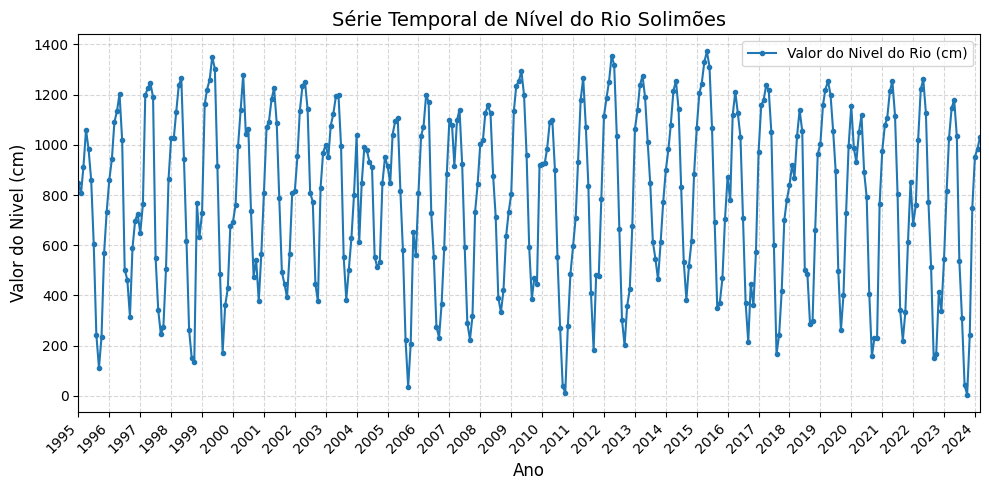
\includegraphics[width=1.0\textwidth]{nivel.png} % Inclui a imagem com 70% da largura do texto
		\caption{Gráfico mostrando o comportamento da série nível 30 anos.} % Legenda da figura
		\label{fig1} % Rótulo para referência cruzada
	\end{figure}
	
	Ao decompor a série nível nos componentes de tendência, sazonalidade e resíduos, Figura \ref{fig2}, temos como primeiras característica para a modelagem as informações de que a série não possui evidência de tendência, possui evidência de sazonalidade e os resíduos são um ruído branco.
	 
	 \begin{figure}[h!]
	 	\centering % Centraliza a imagem
	 	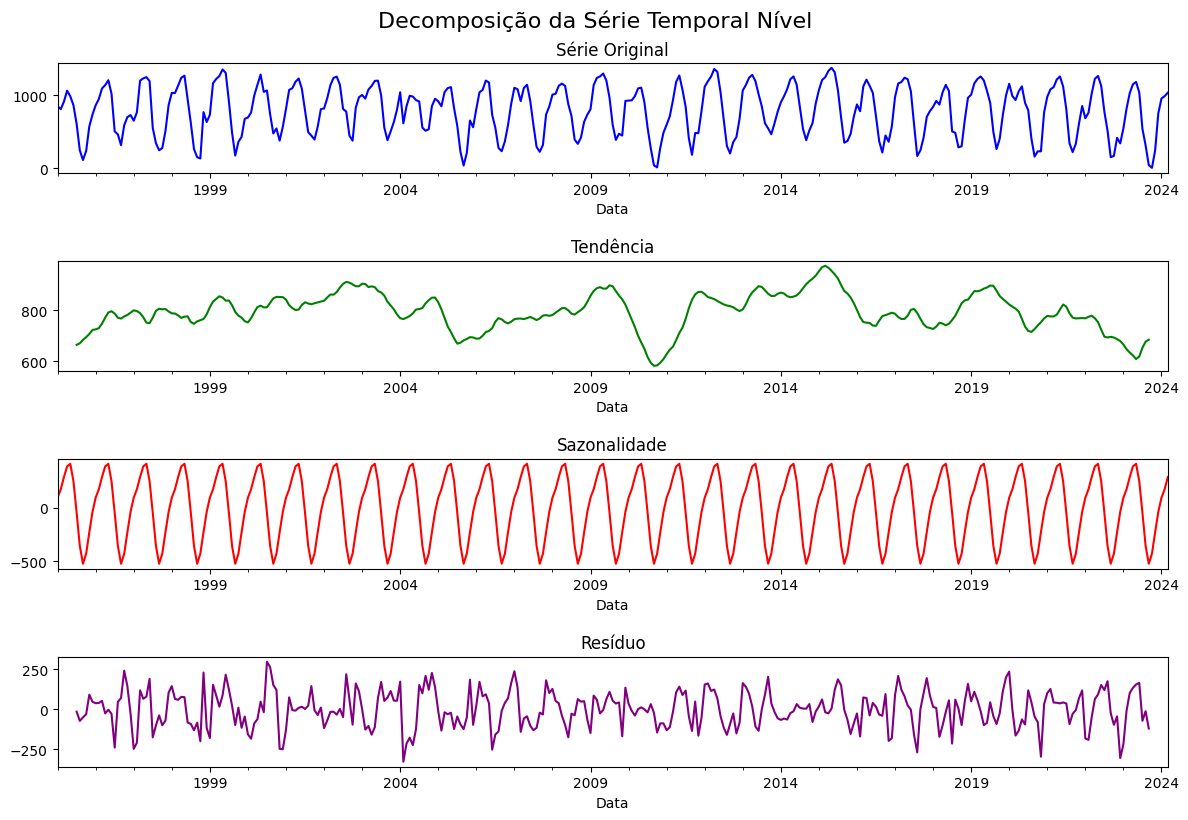
\includegraphics[width=1.0\textwidth]{decomposicao.png} % Inclui a imagem com 70% da largura do texto
	 	\caption{Gráfico mostrando Decomposição da Série Temporal Nível.} % Legenda da figura
	 	\label{fig2} % Rótulo para referência cruzada
	 \end{figure}
	 
	 A evidência de sazonalidade foi confirmada com altíssimo grau de confiança pelo teste de Kruskal-Wallis, com p-valor $\cong 1.78e-55$. Já o teste de Dickey-Fuller aumentado (ADF) confirmou a evidência de estacionariedade da série, apresentando um p-valor = 0.0003.
	 
	O Teste de Dickey-Fuller mostrou que a série já é estacionária (d=0). O Teste de Kruskal-Wallis confirmou a presença de sazonalidade, para ser removido o efeito da sazonalidade e tornar a série sazonalmente estacionária, aplicamos uma diferenciação sazonal (D=1). Os dados são mensais e a sazonalidade em níveis de rios é anual (ciclo de cheias e secas). Portanto, o padrão se repete a cada 12 meses.  Diante desses resultados temos a seguinte configuração inicial do modelo SARIMA(p, 0, q)x(P, 1, Q, 12). 
	 
	 Para determinar os valores para os termos Auto-Regressivos (p, P) e de Média Móvel (q, Q), analisamos os gráficos de Função de Autocorrelação (ACF) e Função de Autocorrelação Parcial (PACF) depois de aplicar a diferenciação sazonal definida (D=1).
	 
	 \begin{figure}[h!]
	 	\centering % Centraliza a imagem
	 	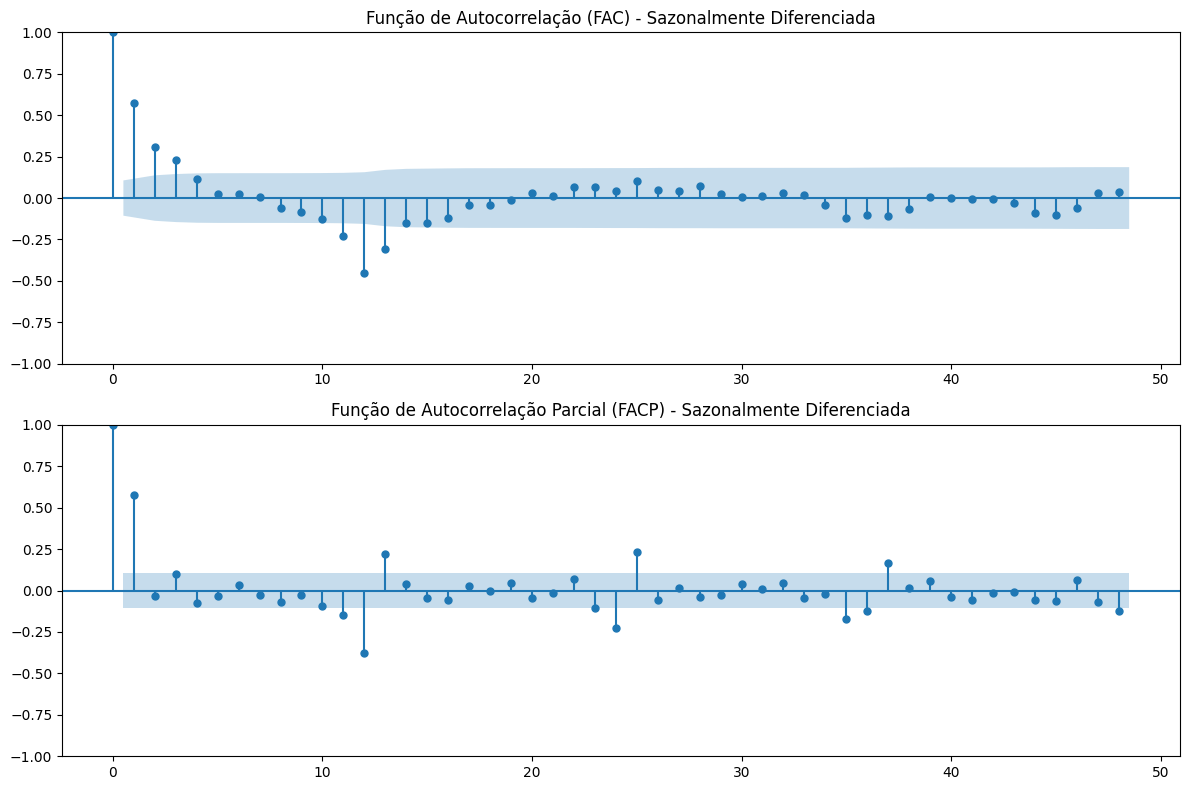
\includegraphics[width=1.0\textwidth]{fac.png} % Inclui a imagem com 70% da largura do texto
	 	\caption{Gráfico mostrando Decomposição da Série Temporal Nível.} % Legenda da figura
	 	\label{fig3} % Rótulo para referência cruzada
	 \end{figure}
	 
	 Analisando a Figura \ref{fig3} temos que o lag onde o gráfico FACP corta para zero (entra na área azul) pela primeira vez é o 2, assim p=2. O valor de q é o lag onde o gráfico FAC corta para zero (entra na área azul) pela primeira vez, ou seja, q=4. Os valores de P e Q são 1, pois é o lag sazonal (12, 24...) onde o FACP e o FAC cortam para zero. Portanto, o modelo incial  é o SARIMA(2, 0, 4)x(1, 1, 1, 12).
	 
	 O modelo escolhido foi implementado pela função do python \textit{sm.tsa.SARIMAX()} da biblioteca $statsmodels$. No output do modelo nos deparamos com a mensagem "\textit{Maximum Likelihood optimization failed to converge}", ou seja, o modelo falhou na convergência. Isso indica que o algoritmo de otimização não conseguiu encontrar os melhores parâmetros possíveis para o modelo. Esse é um resultado que pode ocorrer, já que a técnica de escolhas dos parâmetros não é exata.
	 
	 Realizamos outros testes para a configuração do modelo e o que melhor performou foi o SARIMAX(1, 0, 0)x(1, 1, 0, 12) com tratamento de outlier, cujo resultados estão na Tabela \ref{tab2:sarimax_results}. 
	 
	 \begin{table}[htbp] % Usar [htbp] para mais flexibilidade no posicionamento
	 	\centering
	 	\caption{Resultados do Modelo SARIMAX(1, 0, 0)x(1, 1, 0, 12)}
	 	\label{tab2:sarimax_results}
	 	\small % Reduz o tamanho da fonte para evitar que a tabela fique muito larga
	 	
	 	% Tabela de resumo do modelo (agora em uma única tabela para melhor alinhamento)
	 	\begin{tabular}{llll}
	 		\toprule
	 		\multicolumn{4}{c}{\textbf{Resultados SARIMAX}} \\
	 		\midrule
	 		\textbf{Dep. Variable:}      & nivel                          & \textbf{No. Observations:} & 347                \\
	 		\textbf{Model:}              & SARIMAX(1, 0, 0)x(1, 1, 0, 12) & \textbf{Log Likelihood}    & -1471.851          \\
	 		\textbf{Date:}               & Wed, 30 Jul 2025               & \textbf{AIC}               & 2953.702           \\
	 		\textbf{Time:}               & 10:07:08                       & \textbf{BIC}               & 2972.772           \\
	 		\textbf{Sample:}             & 01-01-1995                     & \textbf{HQIC}              & 2961.304           \\
	 		& - 11-01-2023                   &                            &                    \\
	 		\textbf{Covariance Type:}    & opg                            &                            &                    \\
	 		\bottomrule
	 	\end{tabular}
	 	
	 	\medskip % Adiciona um pequeno espaço vertical
	 	
	 	% Tabela de coeficientes corrigida (7 colunas)
	 	\begin{tabular}{lrrrrrr} % CORRIGIDO: de lrrrrr para lrrrrrr
	 		\toprule
	 		& \textbf{coef} & \textbf{std err} & \textbf{z} & \textbf{P>|z|} & \textbf{[0.025} & \textbf{0.975]} \\
	 		\midrule
	 		\textbf{vazao} & 0.0260 & 0.000 & 112.486 & 0.000 & 0.026 & 0.026 \\
	 		\textbf{outlier\_2013-09-01} & 162.5313 & 17.551 & 9.260 & 0.000 & 128.132 & 196.931 \\
	 		\textbf{ar.L1} & 0.6292 & 0.039 & 16.277 & 0.000 & 0.553 & 0.705 \\
	 		\textbf{ar.S.L12} & -0.4007 & 0.052 & -7.652 & 0.000 & -0.503 & -0.298 \\
	 		\textbf{sigma2} & 449.8358 & 35.365 & 12.720 & 0.000 & 380.522 & 519.150 \\
	 		\bottomrule
	 	\end{tabular}
	 	
	 	\medskip % Adiciona um pequeno espaço vertical
	 	
	 	% Tabela de testes estatísticos
	 	\begin{tabular}{llll}
	 		\toprule
	 		\textbf{Ljung-Box (L1) (Q):} & 0.04 & \textbf{Jarque-Bera (JB):} & 15.28 \\
	 		\textbf{Prob(Q):}            & 0.84 & \textbf{Prob(JB):}         & 0.00 \\
	 		\textbf{Heteroskedasticity (H):} & 1.31 & \textbf{Skew:}             & -0.06 \\
	 		\textbf{Prob(H) (two-sided):} & 0.16 & \textbf{Kurtosis:}         & 4.04 \\
	 		\bottomrule
	 	\end{tabular}
	 	
	 	\medskip
	 	
%	 	\begin{flushleft}
%	 		\footnotesize
%	 		\textbf{Warnings:}\\
%	 		{[1]} Covariance matrix calculated using the outer product of gradients (complex-step).
%	 	\end{flushleft}
	 	
	 \end{table}
	 
	 
	 Para cada coeficiente do modelo (como ar.L1, vazao, etc.), a fórmula para calcular o \textbf{intervalo de confiança} é:
	 
	 
	 $$IC=coef \pm z \times (std\quad err)$$
	 
	 onde:
	 \begin{itemize}
	 
	 
	 	\item coef: É o valor do coeficiente que o modelo estimou (a coluna coef na tabela).
	 	\item std err: É o erro padrão daquela estimativa (a coluna std err). Ele mede a incerteza ou a precisão da estimativa do coeficiente.
		\item  z: É o valor crítico da distribuição Normal padrão. Para um intervalo de confiança de 95\%, o valor de z é aproximadamente 1.96.
	\end{itemize}
	Como resultados temos: 
	
	\begin{itemize}
		\item O coeficiente da variável exógena vazão foi de 0.0260, ou seja, para cada aumento de 1 unidade na vazão, o modelo prevê um aumento de 0.0260 unidades no nível, assumindo que todos os outros fatores permaneçam constantes. Como p-valor = 0.000 e o intervalo de confiança [0.026, 0.026], a vazão é um preditor extremamente forte e confiável para o nível.
		
		\item A variável exógena dummy (outlier\_2013-09-01) mostrou que no mês específico de setembro de 2013, o nível foi, em média, 162.53 unidades mais alto do que o esperado pelo modelo com base apenas na vazão e nos padrões sazonais e de autocorrelação. O p-valor = 0.000 confirma que este pico foi um evento estatisticamente significativo e não um acaso. O intervalo de confiança [128.132, 196.931] mostra que, com 95\% de certeza, o impacto real deste outlier foi um aumento entre 128 e 197 unidades. Isso justifica plenamente a inclusão desta variável para "isolar" o evento.
		
		\item A memória de curto prazo da série representada pelo componente autorregressivo não sazonal (ar.L1) foi de 0.6292. Isso significa que o valor do nível em um mês está positivamente correlacionado com o valor do nível do mês anterior. Cerca de 63\% do valor do resíduo do mês passado é carregado para o mês atual. O p-valor de 0.000 indica que essa dependência do mês anterior é uma característica real e importante da série temporal.
		
		\item A memória de longo prazo, o componente autorregressivo sazonal (ar.S.L12), teve como resultado -0.4007. O coeficiente negativo indica que o valor do nível em um determinado mês está negativamente correlacionado com o valor do nível do mesmo mês no ano anterior, após controlar os outros fatores. Por exemplo, se janeiro deste ano foi mais alto que o esperado, o modelo prevê que o próximo janeiro será ligeiramente mais baixo que o esperado, sugerindo um padrão sazonal oscilatório ou de reversão à média.
		O p-valor de 0.000 confirma que essa relação sazonal de 12 meses é estatisticamente significativa.
		
		\item A variância dos resíduos resultou em 449.8358
		Interpretação: Esta é a estimativa da variância dos erros do modelo. É uma medida do ruído ou da variabilidade que o modelo não consegue explicar. A raiz quadrada deste valor, 
		$\sqrt{449.84} \approx 21.21$, é o desvio padrão dos resíduos. Isso significa que o erro de previsão do modelo é de aproximadamente ±21.21 unidades.
		O p-valor testa se a variância é significativamente diferente de zero, o que é esperado. O valor em si é usado para construir os intervalos de confiança das previsões.
	\end{itemize}
	
	Portanto, o modelo é parcimonioso e bem especificado. Nos informa que o nível de um mês é fortemente influenciado pela vazão (relação positiva), pelo seu próprio valor no mês anterior (inércia positiva), e pelo seu valor no mesmo mês do ano anterior (relação negativa/oscilatória). Além disso, reconhece e quantifica com sucesso um evento anômalo em setembro de 2013, que causou um aumento atípico de cerca de 162.5 unidades.
	
	
	Em relação aos \textbf{testes de hipóteses} de Diagnóstico dos Resíduos temos:
	
	\begin{itemize}
		\item Teste de Autocorrelação (Ljung-Box (Q) e Prob(Q)) verifica se os resíduos são independentes uns dos outros, ou seja, se não há correlação serial nos erros. Apresentou 
		 p-valor de 0.84, muito maior que o nível de significância padrão de 0.05. Portanto, não temos evidências para rejeitar a hipótese de independência dos resíduos.
		Isso confirma o que vimos no gráfico do correlograma. O modelo foi bem-sucedido em extrair toda a informação de correlação temporal dos dados. Os erros remanescentes são aleatórios e não previsíveis, que é exatamente o que se deseja.
		
		\item  Teste de Homocedasticidade ((H) e Prob(H)) verifica se a variância dos resíduos é constante ao longo do tempo. O p-valor de 0.16 é maior que 0.05. Portanto, não rejeitamos a hipótese de variância constante, ou seja, a variabilidade dos erros do modelo é estável ao longo de todo o período analisado (1995-2023). Esta é uma suposição importante para a validade dos intervalos de confiança dos coeficientes.
		
		\item Teste de Normalidade (Jarque-Bera (JB), Prob(JB), Skew e Kurtosis). Este conjunto de métricas trabalha em conjunto para avaliar se os resíduos seguem uma distribuição normal.
		O teste Jarque-Bera (JB) testa formalmente a hipótese de normalidade. Seu p-valor é 0.00, o que nos leva a rejeitar a hipótese nula, isto é, os resíduos não seguem uma distribuição normal. Olhando para as outras duas métricas, temos que o Skew de -0.06 é extremamente próximo de 0. Isso significa que a distribuição dos erros é quase perfeitamente simétrica. A Kurtosis de 4.04 é maior que o valor de 3 de uma distribuição normal. Na prática, isso significa que a distribuição dos erros tem um pico mais acentuado e caudas mais pesadas do que a normal, ou seja, há uma probabilidade ligeiramente maior de ocorrerem erros extremos (outliers) do que o esperado.
		Embora a normalidade seja formalmente rejeitada, a causa é uma curtose um pouco elevada, e não uma assimetria. Para fins de previsão, muitos modelos de séries temporais são robustos a pequenas violações da normalidade, especialmente quando as outras suposições (independência e homocedasticidade dos erros) são atendidas.
		
		
	\end{itemize}
	
	Para reforçar a análise desses resultados apresentamos Figura \ref{fig5} o gráfico dos diagnósticos dos resíduos.
	
	\begin{figure}[h!]
		\centering % Centraliza a imagem
		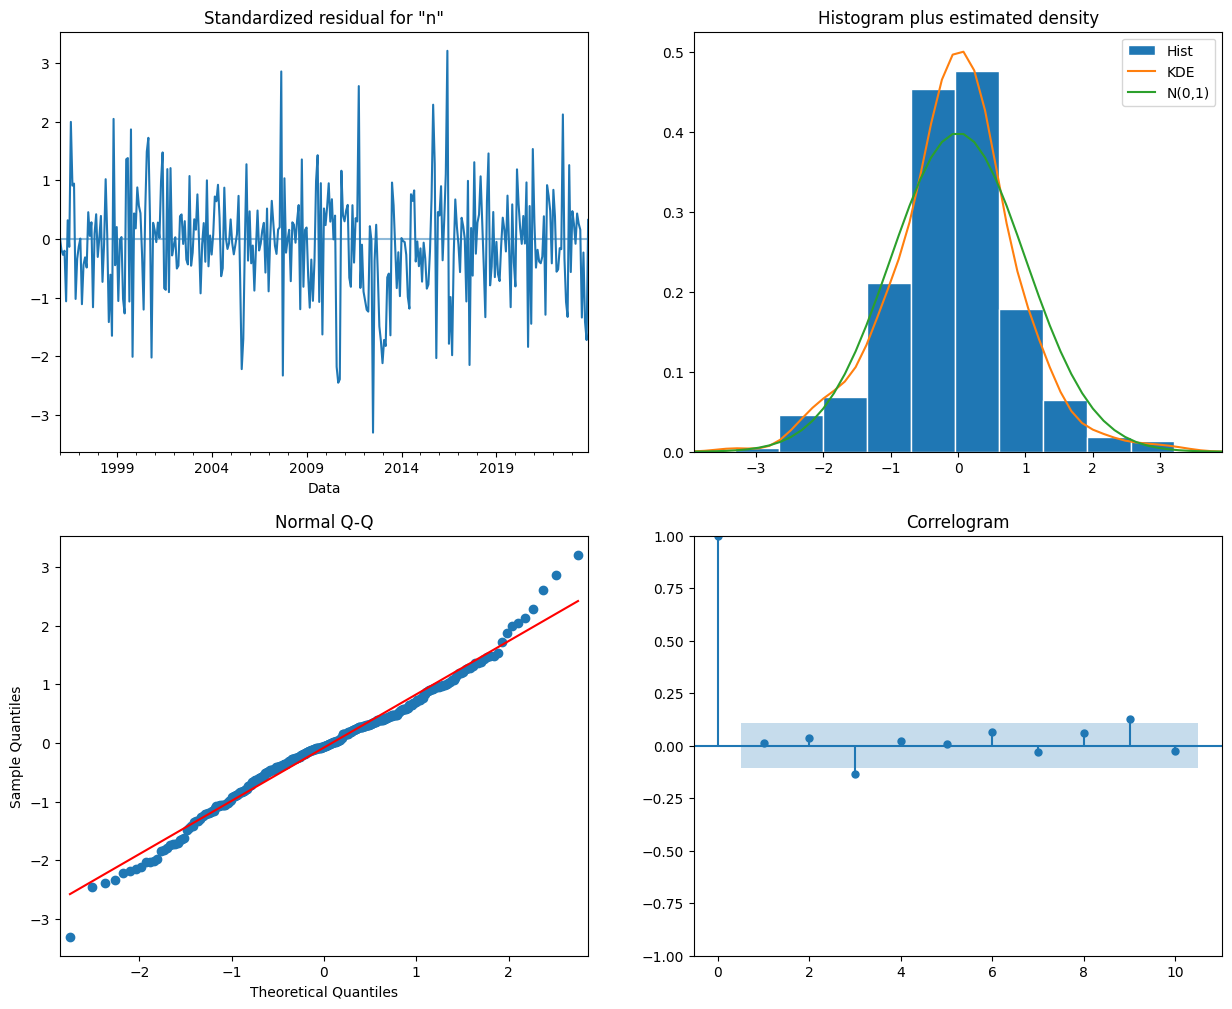
\includegraphics[width=0.8\textwidth]{residuos.png} % Inclui a imagem com 70% da largura do texto
		\caption{Gráfico dos Diagnósticos dos Resíduos} % Legenda da figura
		\label{fig5} % Rótulo para referência cruzada
	\end{figure}
	
	Usando os dados das variáveis exógenas do conjunto de teste, ou seja, os valores dos últimos 4 meses e o modelo treinado geramos as previsões para os meses de dezembro de 2023 a março de 2024. Temos na Figura \ref{fig4} na primeira parte do gráfico os dados reais na cor azul e o ajuste do modelo sobre os dados de treino na cor vermelha, o que mostra quão bem o modelo aprendeu os padrões dos dados de treino. Na segunda parte, de cor verde são os dados reais, de cor vermelha os valores previstos utilizando os valores das variáveis exógenas dos dados de teste e a área sombreada (rosa) em torno da linha de previsão a incerteza da previsão. Como a linha verde (dados reais de teste) está sempre contida dentro desta faixa rosa isso significa que o modelo é bom.
	\begin{figure}[h!]
		\centering % Centraliza a imagem
		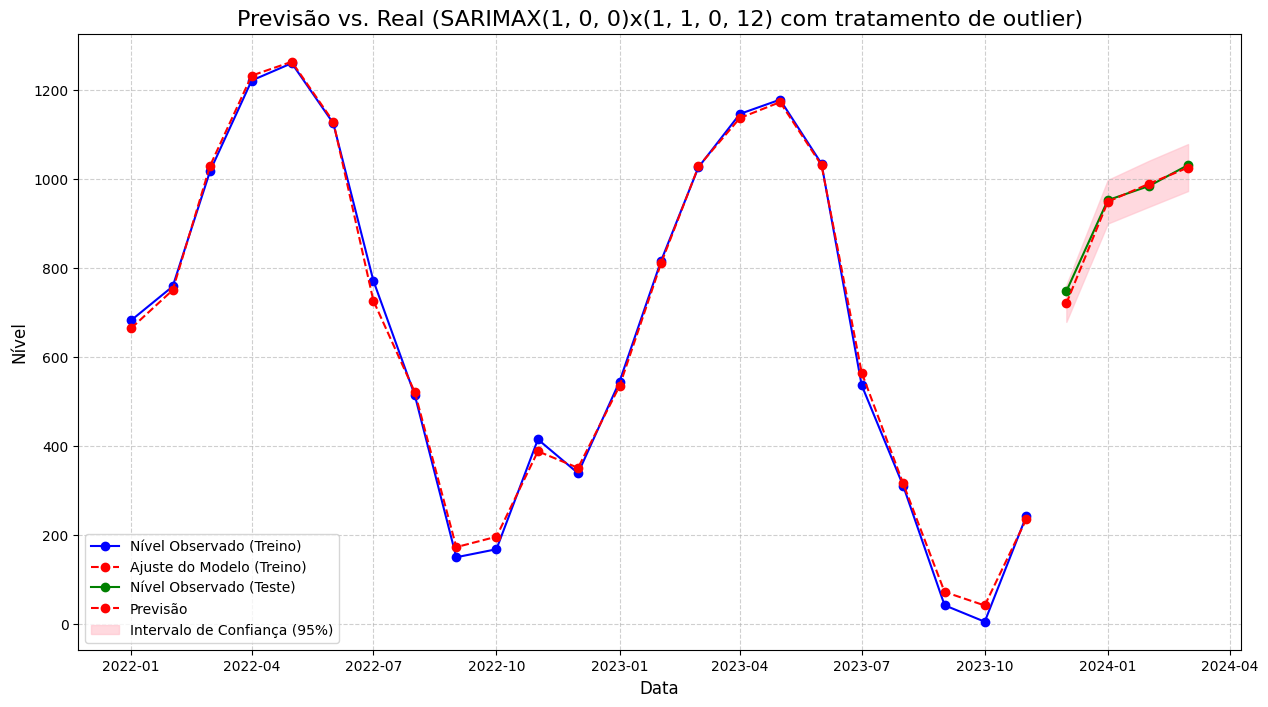
\includegraphics[width=0.8\textwidth]{previsao.png} % Inclui a imagem com 70% da largura do texto
		\caption{Gráfico mostrando Previsão vs. Real da Série Temporal Nível.} % Legenda da figura
		\label{fig4} % Rótulo para referência cruzada
	\end{figure}
	
		Para justificar o uso do modelo 'complexo' fizemos uma comparação com modelos de abordagem ingênua a saber: Previsão Ingênua, a previsão para amanhã é o valor de hoje; Previsão Ingênua Sazonal, a previsão para este mês é o valor do mesmo mês no ano anterior; Média, a previsão é simplesmente a média de todos os dados históricos de treino.
		
	\begin{table}[htbp]
		\centering
		\caption{Comparação de Métricas de Erro entre o Modelo SARIMAX e Baselines}
		\label{tab:model_comparison}
		\begin{tabular}{lrrr}
			\toprule
			\textbf{Modelo} & \textbf{RMSE} & \textbf{MAE} & \textbf{MAPE (\%)} \\
			\midrule
			\textbf{SARIMAX} & \textbf{14.27} & \textbf{10.41} & \textbf{1.27} \\
			\addlinespace % Adiciona um pequeno espaço para separar os modelos
			--- Baselines --- & & & \\
			\addlinespace
			Ingênuo & 696.01 & 687.50 & 73.56 \\
			Ingênuo Sazonal & 300.97 & 247.75 & 28.78 \\
			Média & 177.82 & 161.20 & 16.55 \\
			\bottomrule
		\end{tabular}
		%\begin{flushleft}
%			\footnotesize
%			\textbf{Nota:} RMSE (Root Mean Squared Error), MAE (Mean Absolute Error), MAPE (Mean Absolute Percentage Error). Valores menores indicam melhor desempenho.
%		\end{flushleft}
	\end{table}
	

	
	O resultado desta comparação está apresentada na Tabela \ref{tab:model_comparison} e confirma que o modelo SARIMAX proposto tem um bom desempenho.
	
	
	
	
	\section{Discussão}
	%O modelo desenvolvido representa um equilíbrio bem-sucedido entre ajuste e parcimônia, conforme indicado pelos baixos valores de AIC e BIC. 
	A principal força do modelo reside na sua estrutura abrangente, que não apenas modela a dinâmica intrínseca da série (tendência e sazonalidade), mas também incorpora o efeito de uma variável externa (vazao) e isola o impacto de eventos extremos através de dummies.
	
	A questão da não normalidade dos resíduos merece uma análise aprofundada. Embora o teste de Jarque-Bera tenha falhado, isso não invalida necessariamente o modelo para fins de previsão. Este resultado sugere que a distribuição real dos choques aleatórios na série hidrológica é inerentemente de cauda pesada (leptocúrtica) em comparação com uma distribuição gaussiana. Mesmo após a remoção do outliers mais estatisticamente significativo, a distribuição dos erros remanescentes ainda se desvia da normalidade. Tentar corrigir isso adicionando mais dummies levaria a um modelo excessivamente complexo (overfitting) com ganhos marginais.
	
	%Adicionalmente, o aviso de "matriz singular" observado durante o ajuste é interpretado como um artefato numérico da alta colinearidade introduzida pelas dummies, que explicam perfeitamente a variância em pontos específicos. Dado que a origem do aviso é compreendida e os coeficientes são teoricamente sólidos, ele pode ser considerado com segurança.
	
	Portanto, o modelo é considerado robusto. A ausência de autocorrelação nos resíduos garante que as previsões não serão sistematicamente viesadas, e a homocedasticidade garante que a incerteza da previsão (intervalo de confiança) é estimada de forma confiável.
	
	\section{Conclusões}
	Este trabalho demonstrou a construção bem-sucedida de um modelo SARIMAX para a previsão de níveis de rio. O modelo final, $SARIMAX(1,0,0)(1,1,0)_{12}$, ajustado sobre dados e incluindo a vazão e dummie de outlier como variáveis exógenas, provou ser eficaz.
	
	O modelo passou nos testes diagnósticos críticos de autocorrelação e heterocedasticidade, validando sua estrutura para fins de previsão. A falha no teste de normalidade dos resíduos foi interpretada não como uma deficiência do modelo, mas como uma característica intrínseca dos dados hidrológicos.
	Conclui-se que o modelo desenvolvido é uma ferramenta poderosa e estatisticamente defensável, capaz de gerar previsões confiáveis e fornecer insights valiosos sobre a dinâmica do sistema do reservatório.
	
	Como passos futuros, destacamos buscar compará-lo com resultados de modelos com mesmo propósito presentes na literatura  e testa o modelo mais relaxado considerando erros não normais.
	

	
		
%	\addbibresource{referencias} % Nome do seu arquivo .bib
\printbibliography[title={Referências}]
%		\bibliography{referencias}
	\end{document} % Este é o fim do documento
